\documentclass[../../../include/open-logic-section]{subfiles}

\begin{document}

\olfileid{sth}{ordinals}{idea}	
\olsection{اندیشهٔ کلیِ عدد ترتیبی}

اعداد طبیعی را با ترتیب معمولشان در نظر بگیرید:
\begin{center}
	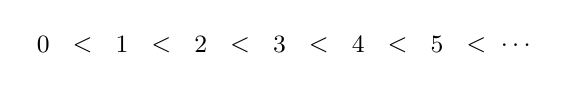
\begin{tikzpicture}
	\foreach \x/\xtext in {0, 1, 2, 3, 4, 5}
	{
		\node (\x a) at (\x, 1) {\small{$\x$}};
		\node (\x a) at (\x.5, 1) {\small{$<$}};
	}
	\node (ldots) at (6, 1) {\small{$\ldots$}};
	\end{tikzpicture}
\end{center}
در اصطلاح فنی، این را یک دنبالهٔ~$\omega$ می‌نامیم. و در واقع، این ترتیب
کلی در ساخت آغازین ما از مراحل سلسله‌مراتب مجموعه‌ها بازتاب یافته است.
اما اکنون فرض کنید~$0$ را به انتهای این دنباله ببریم، به‌طوری‌که پس از
همهٔ عددهای دیگر قرار گیرد:
\begin{center}
	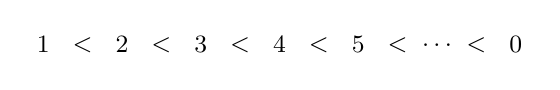
\begin{tikzpicture}
	\foreach \x/\xtext in {1, 2, 3, 4, 5}
	{
		\node (\x a) at (\x, 1) {\small{$\x$}};
		\node (\x a) at (\x.5, 1) {\small{$<$}};
	}
	\node (ldots) at (6, 1) {\small{$\ldots$}};
	\node (bea) at (6.5, 1) {\small{$<$}};
	\node (noa) at (7, 1) {\small{$0$}};
	\end{tikzpicture}
\end{center}
اینجا همان موجودات را داریم، اما به شیوه‌ای اساساً متفاوت مرتب شده‌اند:
ترتیب نخست ما هیچ عضو آخری نداشت، ولی ترتیب تازه‌مان دارد. در واقع، ترتیب
تازه از یک دنبالهٔ~$\omega$ از موجودات
($1,2,3,4,5,\ldots$) تشکیل شده که موجودی دیگر پس از آن آمده است. پس این
یک دنبالهٔ~$\omega+1$ خواهد بود.

تنها با همین موجودات می‌توانیم انواع بیشتری از ترتیب را پدید آوریم. برای
نمونه، همهٔ اعداد زوج (با ترتیب طبیعی‌شان) و سپس همهٔ اعداد فرد (با ترتیب
طبیعی‌شان) را در نظر بگیرید:
\begin{center}
	\begin{tikzpicture}
	\node(a1) at (1,1) {\small{$0$}};
	\node(a2) at (1.5,1) {\small{$<$}};
	\node(a3) at (2,1) {\small{$2$}};
	\node(a4) at (2.5,1) {\small{$<$}};
	\node(a5) at (3,1) {\small{$4$}};
	\node(a6) at (3.5,1) {\small{$<$}};
	\node(dots) at (4,1) {\small{$\ldots$}};
	\node(aaoe) at (4.5,1) {\small{$<$}};
	\node(b1) at (5,1) {\small{$1$}};
	\node(b2) at (5.5,1) {\small{$<$}};
	\node(b3) at (6,1) {\small{$3$}};
	\node(b4) at (6.5,1) {\small{$<$}};
	\node(b5) at (7,1) {\small{$\ldots$}};
	\end{tikzpicture}
\end{center}
این یک دنبالهٔ~$\omega$ است که دنبالهٔ~$\omega$ دیگری پس از آن آمده؛ یعنی
یک دنبالهٔ~$\omega+\omega$.

البته می‌توانیم همچنان ادامه دهیم. اما آنچه می‌خواهیم روشی کلی برای فهم
این سخن دربارهٔ \emph{ترتیب‌ها} است.

\end{document}
